\section{Scelte implementative}
\label{cap:implementation-choices}

\subsection{Rappresentazione del grafo}
\label{sub:graph-representation}

Gli algoritmi di questo homework operano su grafi pesati completamente connessi e non diretti. Ha quindi senso rappresentare ogni grafo con una Matrice di Adiacenza, dato che i grafi sono completi. In questa relazione useremo in maniera ambivalente i termini \textit{Matrice di Adiacenza} e \textit{Matrice delle distanze}, poiché i grafi sono pesati.

\noindent I dataset contenenti i grafi di input sono in formato standard \textbf{TSPLIB } e riportano le coordinate 2D dei nodi del grafo in due possibili formati:

\begin{itemize}
    \item \textbf{EUC\_2D}: le coordinate rappresentano la posizione nello spazio euclideo a 2 dimensioni. È dunque richiesto il calcolo della distanza euclidea tra ogni nodo, con il valore arrotondato al numero intero più vicino;
    \item \textbf{GEO}: le coordinate rappresentano la latidudine e la longitudine di ogni punto. Il calcolo della distanza tra due punti in questo caso è più complesso, e richiede una conversione preliminari in radianti; rimandiamo alle FAQ della consegna per ulteriori dettagli.
\end{itemize}

\noindent I risultati del calcolo delle distanze (\textit{EUC\_2D} o \textit{GEO} a seconda del dataset di input) sono inseriti nella posizione corrispondente della Matrice delle Distanze.
Una volta calcolate le distanze, le coordinate originali non sono mantenute: non sono infatti necessarie ai fini della rappresentazione del grafo e del calcolo della soluzione di TSP.
Nella figura \ref{fig:distancematrix-example} è possbile vedere un esempio di una conversione di un grafo di esempio rappresentato da cordinate EUC\_2D nella sua matrice delle distanze.

\begin{figure}[h]
	\centering
	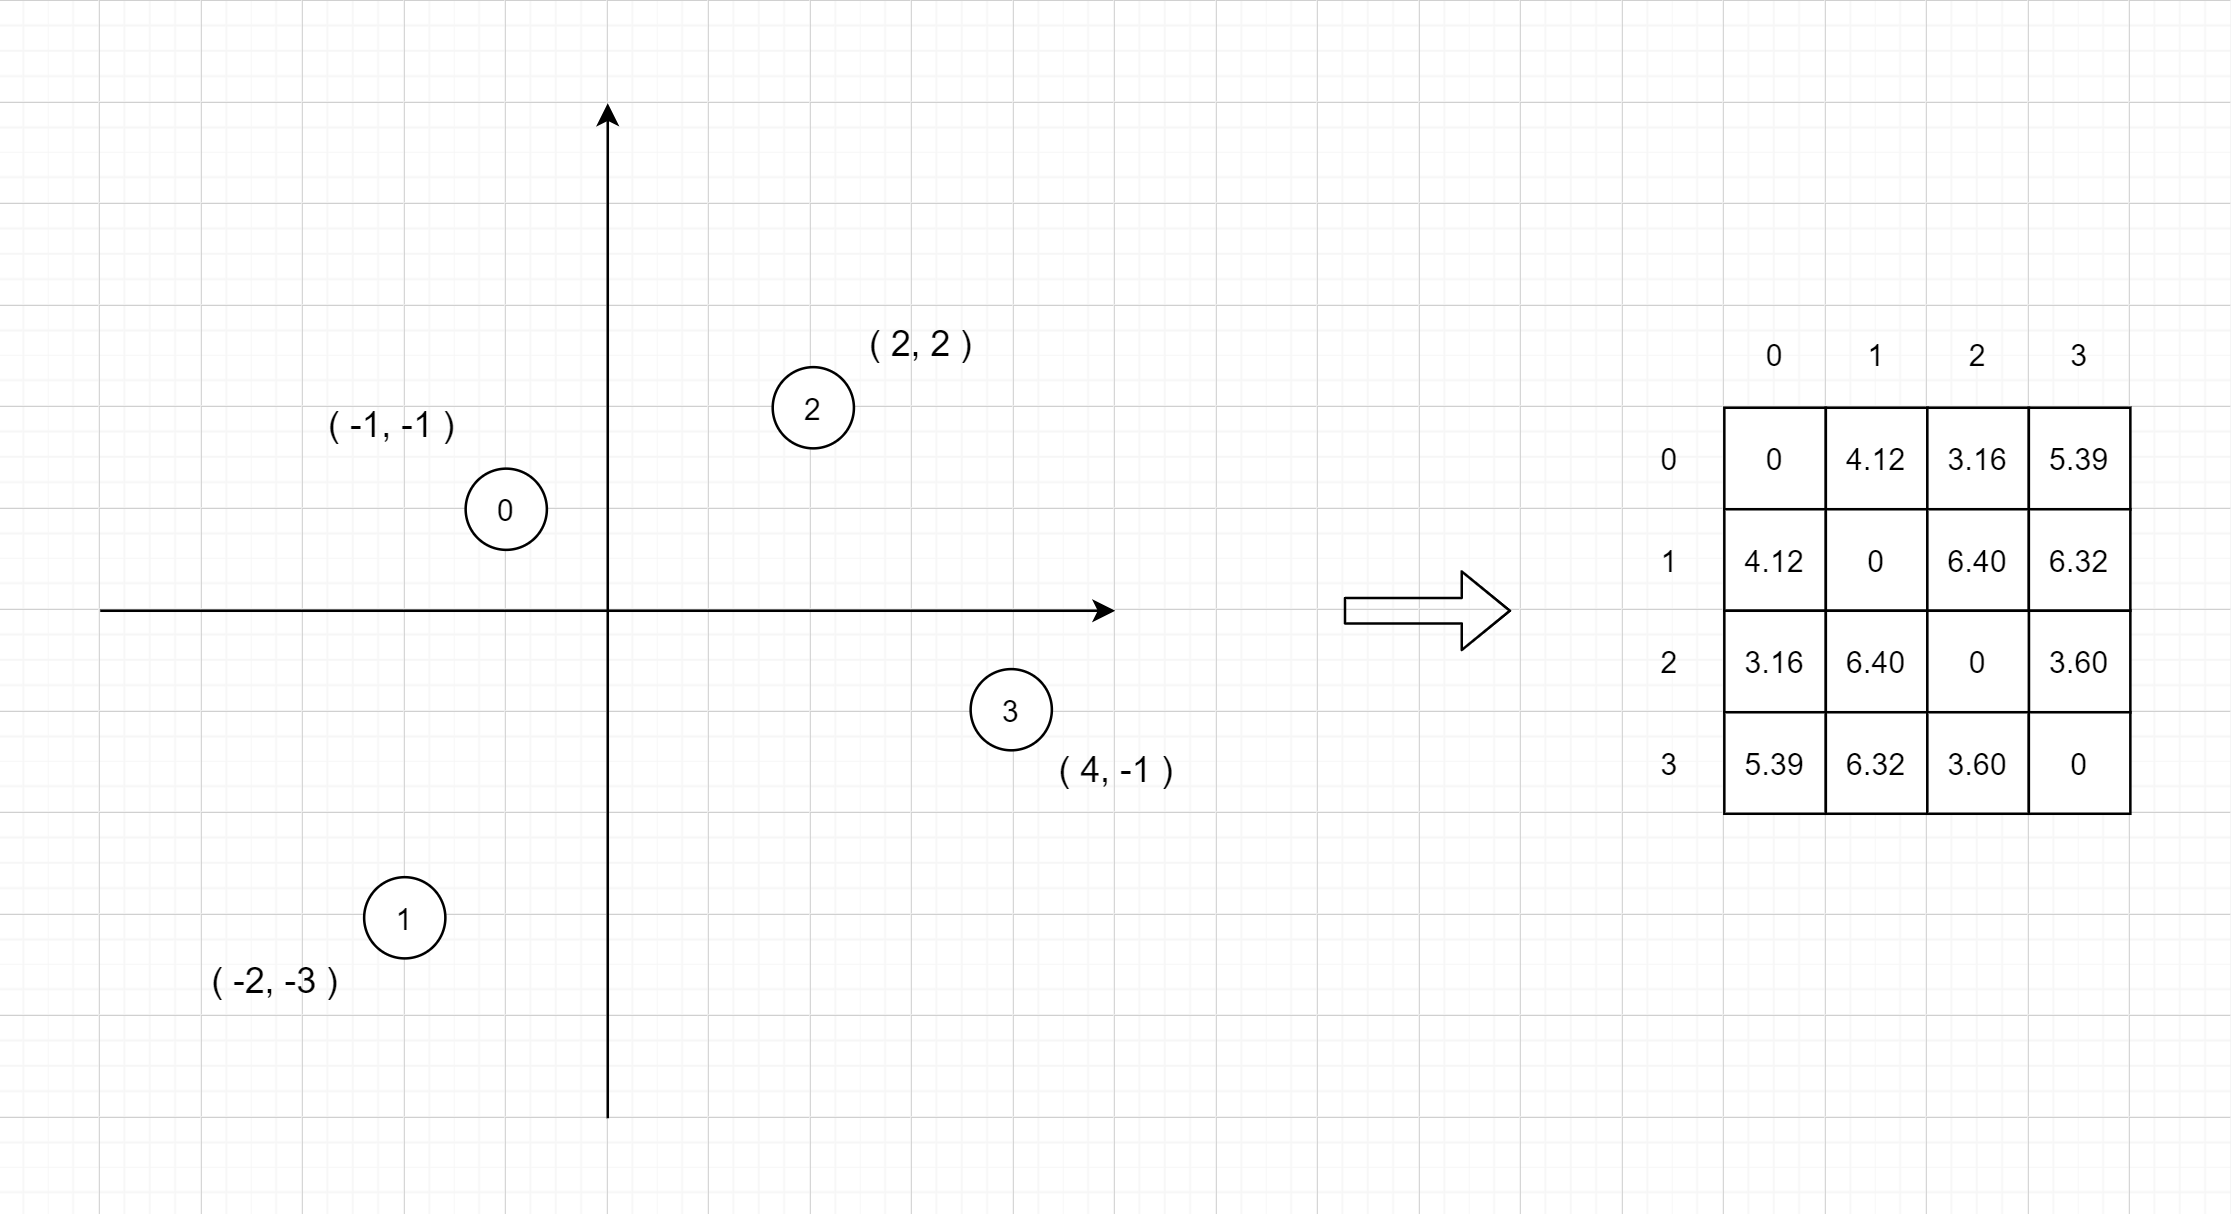
\includegraphics[width=0.9\textwidth]{./images/Distance Matrix.png}
	\caption{Grafo di esempio rappresentato con Matrice delle distanze}
	\label{fig:distancematrix-example}
\end{figure}

\noindent Come nel precedente homework, per semplificare la logica di indicizzazione dei nodi del grafo, la label dei nodi (originariamente numerata da $1$ a $n$) è decrementata di 1, quindi i nodi sono rappresentati dall'intervallo numerico $[0, n-1]$.

\noindent La classe che rappresenta la Matrice delle Distanze dei grafi è definita in \codeinline{DistanceMatrix.h} nella cartella \textit{Shared}.

\begin{listing}[!ht]
\begin{minted}{c++}
std::vector<T> data;

// mappa la coppia di indici (row, column) della matrice in un indice per
// il vettore 1-dimensionale data. (Indicizzazione fisica)
[[nodiscard]] size_t get_index(size_t row, size_t column) const noexcept {
    return row * n_vertexes + column;
}

// valore della distanza tra i nodi (i, j). (Indicizzazione virtuale)
[[nodiscard]] T& at(size_t i, size_t j) noexcept {
    return data.at(get_index(i, j));
}
\end{minted}
\caption{Indicizzazione virtuale e fisica della classe DistanceMatrix.h.}
\label{listing:virtual-physica-addressing}
\end{listing}

\paragraph{Ottimizzazioni}\mbox{} \\

\noindent Poichè i grafi in esame sono non diretti ($\forall i,j \in V$, $c(i,j) = c(j,i)$), la Matrice delle Distanze è una matrice simmetrica con tutte le entry della diagonale principale pari a 0 (in quanto ogni vertice dista 0 da se stesso).
Abbiamo quindi calcolato le distanze \textit{pair-wise} solo per la parte triangolare superiore della matrice, per poi copiarle in maniera trasposta nella parte triangolare inferiore. Questo ci ha permesso quindi di calcolare le stesse distanze più volte. \\

\noindent La matrice è rappresentata da un singolo \codeinline{std::vector}. Questo dà la garanzia che ogni riga della matrice sia definita in sezioni contigue di memoria, riduce l'overhead rispetto ad un approccio \codeinline{std::vector<std::vector>}, e, nonostante la logica di indicizzazione sia un po' più complessa (l'indicizzazione virtuale è a due dimensioni, quella fisica è ad una sola dimensione), il cache behaviour della classe è migliore. Si veda il listing \ref{listing:virtual-physica-addressing}.

\begin{listing}[!ht]
\begin{minted}{c++}
int main(int argc, char** argv) {
    if (argc != 2) {
        std::cerr << "1 argument required: filename" << std::endl;
        exit(0);
    }

    const char* filename = argv[1];

    // legge il grafo completo non diretto dal file di input
    auto point_reader(read_file(filename));

    // crea la matrice di distanza, usando le distanze euclidea o geodesica a seconda del
    // tipo di input
    DistanceMatrix<int>&& distance_matrix = point_reader->create_distance_matrix();

    // calcola il peso della soluzione TSP individuata dall'algoritmo
    const auto total_weight = ...;

    // stampa la soluzione trovata
    std::cout << std::fixed << total_weight << std::endl;
}
\end{minted}
\caption{Scheletro comune ad ogni file \codeinline{main.cpp} del progetto.}
\label{listing:main-cpp}
\end{listing}

\subsection{Lettura del Grafo}

\noindent Il file \codeinline{main.cpp} ha la stessa struttura per ogni algoritmo, si veda il listing \ref{listing:main-cpp}. Ad alto livello, le operazioni svolte sono:

\begin{enumerate}
    \item Lettura del file di input: il file di input viene parsato, e vengono lette solo le informazioni più importanti, ovvero:
    
    \begin{itemize}
        \item dimensione del grafo;
        \item tipo di distanza (\textit{EUC\_2D} o \textit{GEO});
        \item coordinate del grafo.
    \end{itemize}
    
    \noindent Abbiamo usato la libreria di file streaming offerta da C++ (\codeinline{fstream}). Abbiamo rappresentato il tipo di distanza dall'enumerazione \codeinline{EdgeWeightType.h}, per la quale abbiamo definito l'operatore di lettura \codeinline{std::istream\& operator>>}.
    
    \item I punti definiti dopo la riga \textit{NODE\_COORD\_SECTION} del dataset di input sono letti con un'istanza polimorfica di \codeinline{PointReader.h}, che interpreta le coordinate in maniera diversa a seconda del valore assunto dall'enumerazione \codeinline{EdgeWeightType}, ovvero a seconda del tipo di distanza del file. Naturalmente, la sottoclasse \codeinline{EuclideanPointReader.h} usa la distanza Euclidea, mentre \codeinline{GeodesicPointReader.h} usa quella geodesica. Le classi dei punti letti in input sono definiti in \codeinline{point.h} (\codeinline{point\_2D} per le coordinate euclidee, \codeinline{point\_geo} per le coordinate geografiche), e per ognuno di essi è stato definito l'operatore di lettura \codeinline{std::istream\& operator>>} adeguato. Questo ci ha permesso di non avere duplicazione di codice per gestire tipi diversi di punti in input. \\
    
    \noindent La label dei nodi è decrementata di 1 in questa fase di lettura.
    
    \item Una volta letti i nodi, viene creata la matrice delle distanze tramite \textit{Template Method Pattern}, usando la nozione di distanza definita dalle sottoclassi di \codeinline{PointReader.h}. Il metodo concreto \codeinline{distance(i, j)} delle sottoclassi è usato nel costruttore di \codeinline{DistanceMatrix} come \textit{higher-order function}. Si veda il listing \ref{listing:point-reader}.
\end{enumerate}

Tutti i file citati qui sopra sono nella cartella \textit{Shared} del progetto consegnato.

\begin{listing}[!ht]
\begin{minted}{c++}
class PointReader {
protected:
  std::fstream& file;
  size_t dimension;

  // calcola la distanza tra i punti i e j
  virtual int distance(size_t i, size_t j) const = 0;

public:
  PointReader(std::fstream& file, size_t dimension) :
    file(file), dimension(dimension) { }

  virtual ~PointReader() = default;

  // consuma la lista di coordinate dal file di input
  virtual void read() = 0;
    
  // crea la matrice delle distanze a partire dai punti letti. Usa il metodo distance 
  // implementato dalle sotto classi come funzione higher-order
  DistanceMatrix<int> create_distance_matrix() {
    using namespace std::placeholders;
    auto distance_fun(std::bind(&PointReader::distance, this, _1, _2));

    return DistanceMatrix<int>(dimension, distance_fun);
  }
};
\end{minted}
\caption{Definizione parziale di \codeinline{PointReader.h} che evidenza la creazione della matrice delle distanze del grafo letto.}
\label{listing:point-reader}
\end{listing}

\subsection{Strutture Dati}

Tutte le strutture dati elencate di seguito sono definite nella cartella \textit{Shared}.
Ove possibile, per la nomenclatura dei metodi abbiamo cercato di seguire lo stesso standard dei container STL di C++.
Inoltre, le strutture dati usate sono sempre pre-allocate in memoria quando possibile, evitando rehashing e riallocazioni dispendiose. Questo significa che la maggior parte delle operazioni indicate con \complexityConstant{} ammortizzato siano in realtà totalmente costanti nella pratica.

\noindent Le strutture dati relative alle Heap e alle code di priorità necessarie per l'algoritmo di Prim sono già state ampiamente documentate nell'homework 1.

\subsubsection{Rappresentazione dei vettori $\pi$ e $d[v,S]$}

L'algoritmo Held-Karp richiede esplicitamente l'uso di due vettori:
\begin{itemize}
    \item $d[v,S]$ è il peso del cammino minimo che parte da 0 e termina in v, visitando tutti i nodi in S;
    \item $\pi[v,S]$ è il predecessore di v nel cammino minimo definito come sopra.
\end{itemize}

In questo caso l'homework prevede la restituizione del peso del cammino Hamiltoniano inferiore e non il cammino stesso, il vettore $\pi[v,S]$ è stato omesso. Per poter implementare dunque il vettore $d[v,S]$ si è deciso di creare una struttura dati apposita, formata da una \textit{std::unordered\_map} dove la chiave è una coppia $(S, v)$ ed il valore della mappa è un intero che rappresenta il peso del cammino minimo che parte da 0 e termina in v, visitando tutti i nodi in S. Per rappresentare il set di nodi S si sono studiate 3 possibili soluzione descritte nella sezione \ref{cap:S-repr}. Mentre il vertice $v$ viene rappresentato da un numero di tipo \textit{size\_t}.

\subsubsection{Rappresentazione del sottoinsieme di vertici S}
\label{cap:S-repr}
In particolare ora vogliamo concentrare la nostra attenzione alla rappresentazione in maniera efficiente dell'insieme dei nodi S da visitare. In particolare abbiamo pensato a 3 soluzioni che argomenteremo qui di seguito.

\paragraph{Unordered Set}
La prima soluzione è quella di rappresentare il set di vertici S semplicemente attraverso la struttura dati \textit{unordered\_set} offerta dalla standard library \textit{std} di C++.  

TODO: PARLARE DELL'HASHING

\paragraph{Bitmasking}

\noindent Una soluzione migliore per rappresentare il set di nodi S visitati in maniera compatta è usare un numero a 64 bit (assumendo di non considerare le architetture a 32 bit). In questo caso ogni bit rappresenta la presenza o meno nel set S del vertice $i$ dell'$i$-esimo bit considerato nel numero. Per fare questo è stato sufficiente dichiarare un numero \textit{unsigned long long} che nel nostro linguaggio corrisponde ad numero senza segno a 64 bit. Tale numero viene manipolato sfruttando la sua rappresentazione binaria per decretare la presenza o meno dell'$i$-esimo vertice. Si consideri l'esempio in figura \ref{fig:bitmasking-example}, è possibile vedere come è possibile rappresentare l'insieme S attraverso i bit di un numero unsigned long long. 

\begin{figure}[h]
	\centering
	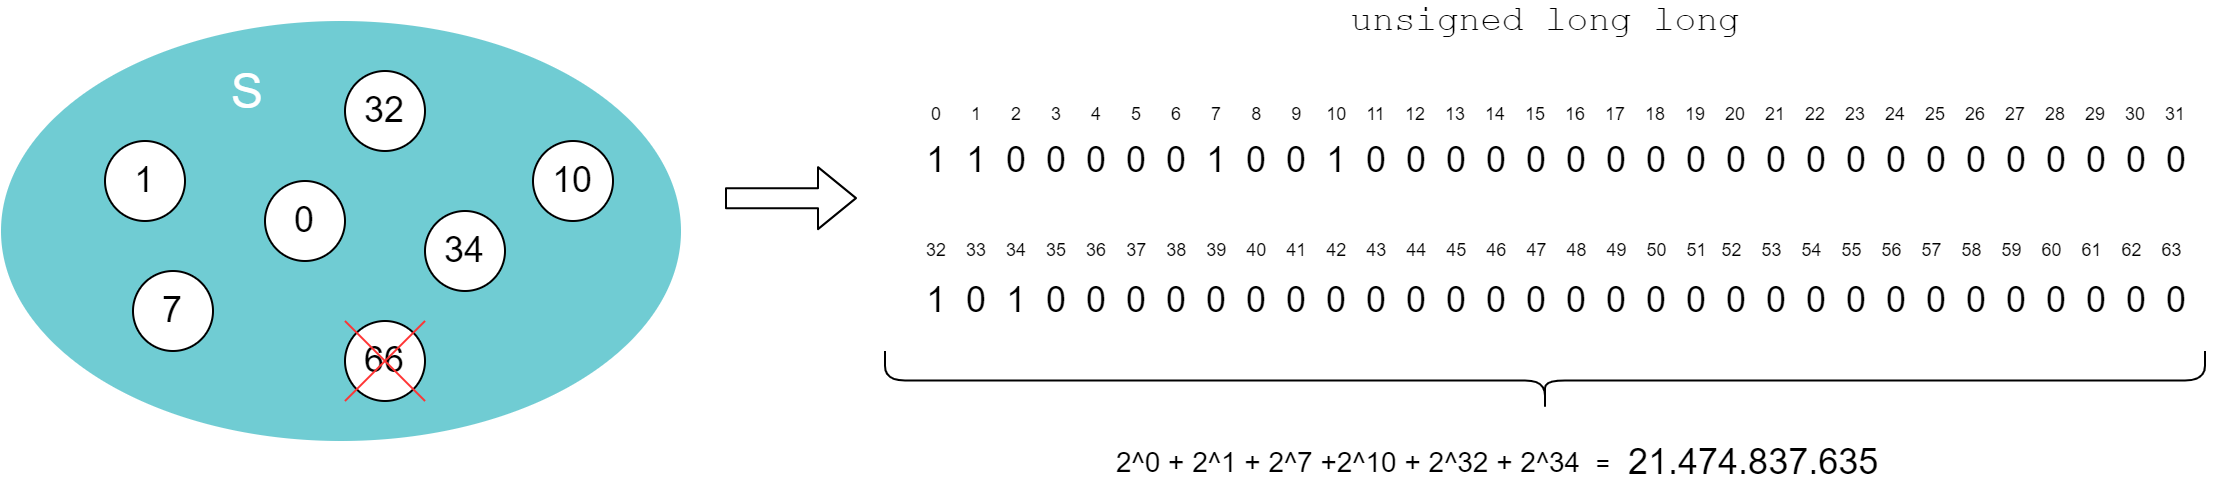
\includegraphics[width=0.9\textwidth]{./images/BitMasking Example.png}
	\caption{Rappresentazione di S tramite BitMasking}
	\label{fig:bitmasking-example}
\end{figure}

Sfruttando questa rappresentazione dell'insieme S, le operazioni di eliminazione, aggiunta e di presenza di nodi sono implementate sfruttando operazioni sui bit tramite tecniche di bit-shifting, operazione logiche AND, OR e NOT: operazione pressoché istantanee nel nostro linguaggio garantendo così un complessità temporale molto bassa.

Un limite di tale struttura è l'impossibilità di poter rappresentare un set S che contiene più di 64 nodi, come è possibile vedere nell'esempio della figura \ref{fig:bitmasking-example} dove il vertice 66 non può essere rappresentato in questo modo.

\paragraph{Extended Bitmasking}
TODO: Cambiare nome nel codice da ExtendedBitSet a ExtendedBitMasking.
Per superare il limite della rappresentazione tramite BitMasking per più di 64 nodi si è pensato di estendere l'idea del bitmasking non più ad un solo numero, ma a più numeri. In questo modo se il set S può raggiungere cardinalità più grandi di 64 nodi è possibile rappresentarlo con più di un numero, dove il primo numero rappresenta i primi 64 nodi, il secondo i successivi 64 nodi e così via. Per fare questo abbiamo dichiarato un'apposita classe chiamata \textit{EtendedBitMasking} che tramite un \textit{std::vector} di \textit{unsigned long long} è in grado di rappresentare qualunque set S. In questo modo, data una posizione di un bit $i$, è sufficiente ricavarsi l'indice del vettore dove risiede il numero che contiene il bit $i$ (tramite la divisione intera di $i$ con 64) e la posizione del bit all'interno del numero (tramite il resto della divisione di $i$ con 64). Nell'esempio raffigurato in figura \ref{fig:extendedbitmasking-example} è possibile vedere come lo stesso set S visto nell'esempio precedente ora possa essere rappresentato tramite questa nuova struttura.

\begin{figure}[h]
	\centering
	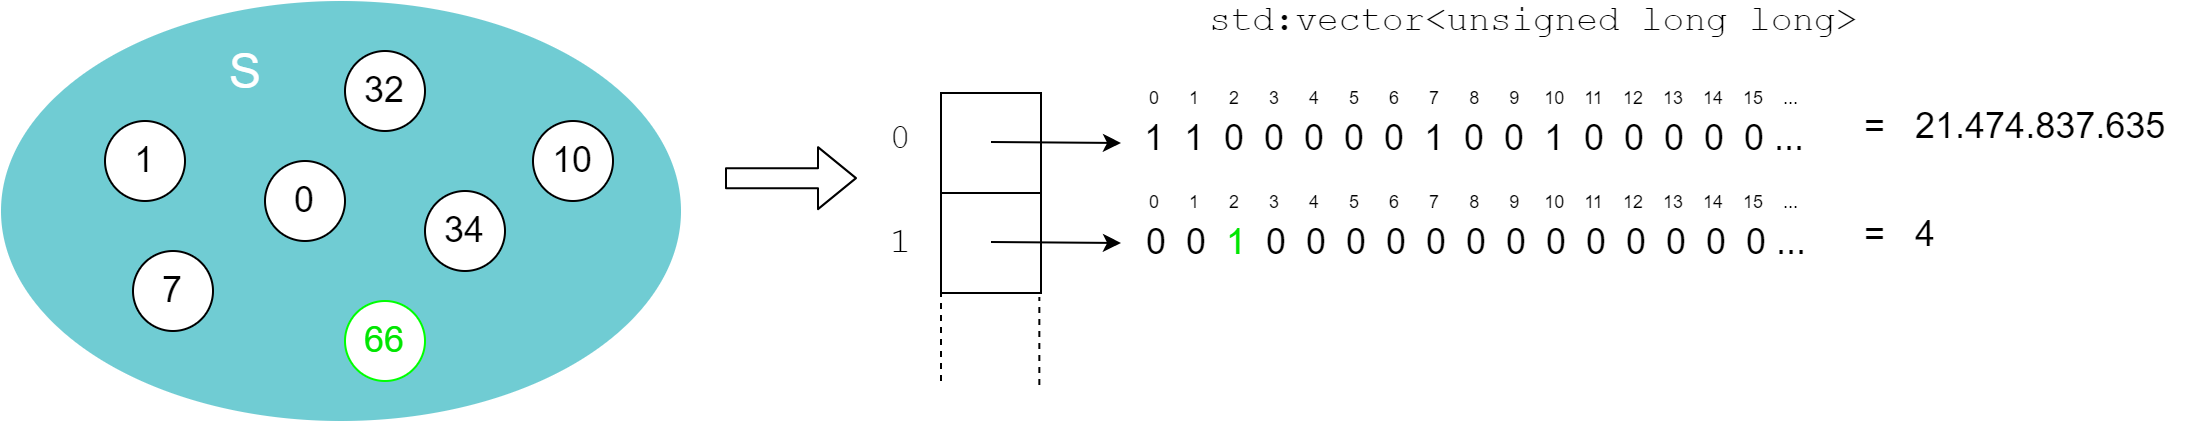
\includegraphics[width=0.9\textwidth]{./images/BitMaskingExtended Example.png}
	\caption{Rappresentazione di S tramite ExtendedBitMasking}
	\label{fig:extendedbitmasking-example}
\end{figure}

\paragraph{Confronto tra unordered\_set, BitMasking ed ExtendedBitMasking}
In questo paragrafo vogliamo mettere a confronto le performance in termini di complessità spaziali e temporali delle 3 soluzioni proposte.

\subsection{Timeout}

\noindent L'algoritmo di Held-Karp ha complessità temporale \complexityHeldKarpTime{}, quindi i tempi di esecuzione \textit{esplodono} anche solo per grafi con poche decine di nodi. Come richiesto dall'homework, all'algoritmo di Held-Karp è assegnato un timeout di esecuzione $T$. Abbiamo fissato il valore di $T$ a 2 minuti, per mantenere la RAM occupata sotto controllo (anche la complessità spaziale dell'algoritmo è esponenziale).\\

\noindent La nostra implementazione di Held-Karp, quindi:

\begin{enumerate}
    \item Ritorna la soluzione esatta se i suoi tempi di esecuzione sono inferiori a 2 minuti, senza aspettare lo scadere del timeout;
    \item Se invece il timeout scade, termina preventivamente la ricorsione e ritorna la migliore soluzione trovata fino a quel momento. A seconda della profondità del call-stack ricorsivo, la soluzione potrebbe essere ritornata qualche secondo dopo lo scadere del timeout.
\end{enumerate}

\noindent C++17 non fornisce soluzione \textit{out-of-the-box} ad alto livello per eseguire funzioni con un limite di tempo. Abbiamo quindi implementato un meccanismo di questo tipo in \codeinline{Shared/timeout.h}, il cui funzionamento ad alto livello è il seguente:

\begin{itemize}
    \item Il thread principale crea un \textit{worker thread} incaricandolo di eseguire Held-Karp sul grafo letto in input. Fa quindi partire il timeout e resta in attesa del risultato del worker thread. Tale risultato sarà disponibile da un \codeinline{std::future}.
    \item Se il worker thread termina prima dello scadere del timeout, il thread principale è immediatamente sbloccato e il risultato della funzione (restituito da \codeinline{std::future::get()}) è ritornato al chiamante.
    \item Se il timeout scade e il worker thread non ha ancora terminato l'esecuzione, il thread principale gli notifica di terminare l'esecuzione il prima possibile. Tale notifica avviene forzando la conclusione di una \codeinline{std::promise} creata dal main thread e data in input alla funzione eseguita incapsulata nella classe \codeinline{timeout\_signal}.
    \item Quando la funzione eseguita si accorge che il tempo a disposizione è scaduto, interrompe la ricorsione e ritorna la migliore soluzione individuata fino a quel momento al chiamante. 
\end{itemize}